\documentclass[fontsize=12pt,paper=a4,twoside]{scrartcl}

\usepackage{booktabs}
\usepackage{float}


% SWP-Präambel
% C 2003-2017 Sebastian Offermann, Rainer Koschke, Karsten Hölscher
% In Zeilen 40 und 41 sind jeweils die aktuellen Daten einzutragen

\usepackage[utf8]{inputenc}     % Kodierung der Tex-Datei
\usepackage[T1]{fontenc}        % Korrekte Ausgabe von Sonderzeichen (Umlaute)
\usepackage[ngerman]{babel}     % Deutsche Einstellungen [ab \begin{document}]

\usepackage{bibgerm}            % Bibliographie
\usepackage{fancyhdr}           % obere Seitenränder gestalten
\usepackage{float}              % Floats Objekte mit [H] festsetzen
\usepackage{graphicx}           % Graphiken als jpg, png etc. einbinden
\usepackage{moreverb}           % zusätzliche verbatim-Umgebungen
\usepackage{pdflscape}          % PDF-Support für landscape
\usepackage[final]{pdfpages}    % Externe PDFs einbinden
\usepackage{stmaryrd}           % zusätzliche Symbole
\usepackage{supertabular}       % Tabellen über Seitenränder hinaus
\usepackage{tabularx}           % Tabellen mit vorgegebener Breite
\usepackage{url}                % setzt URLs schön mit \url{http://bla.laber.com/~mypage}
\usepackage{lscape}

%%% Die Reihenfolge der folgenden Pakete muss beibehalten werden:
%%% varioref, hyperref, cleveref, bookmark
% Verweise innerhalb des Dokuments schick mit " ... auf Seite ... "
% automatisch versehen. Dazu \vref{labelname} benutzen
\usepackage[ngerman]{varioref}  % [vor hyperref für korrekte Verweise]
\usepackage[colorlinks=true, pdfstartview=FitV, linkcolor=blue,
            citecolor=blue, urlcolor=blue, hyperfigures=true,
            pdftex=true]{hyperref} % [vor bookmark wegen der Optionen]
\usepackage[ngerman]{cleveref}
\usepackage{bookmark}

\hyphenation{Arbeits-paket}     % Trennungsregeln

%%% Definitionen
\newcommand{\grad}{\ensuremath{^{\circ}} }
\renewcommand{\strut}{\vrule width 0pt height5mm depth2mm}
\newcommand{\gq}[1]{\glqq{}#1\grqq{}}
\newcommand{\skipInput}[1]{}

%%% Semesterkonstanten
\newboolean{langversion} %Deklaration
\setboolean{langversion}{false} %Zuweisung ist 'false' für Blockkurs
\newcommand{\jahr}[0]{2017} %2017/2018

% erstes Argument: SWP-2, zweites SWP-1
\newcommand{\highlight}[1]{\textcolor{blue}{\textbf{#1}}}
\newcommand{\variante}[2]{\ifthenelse{\boolean{langversion}}{#1}{#2}}
\newcommand{\nurlangversion}[0]%
    {\variante{\highlight{Muss in SWP-2 ausgefüllt werden}}%
              {\highlight{Entfällt in SWP-1}}}
\newcommand{\swp}[0]{Software-Projekt \variante{2}{1}}
\newcommand{\semester}[0]{\variante{WiSe}{SoSe} \jahr}

%%% Formatierungsanpassungen
% Damit Latex nicht zu lange Zeilen produziert:
\sloppy
%Uneinheitlicher unterer Seitenrand:
%\raggedbottom

% Kein Erstzeileneinzug beim Absatzanfang
% Sieht aber nur gut aus, wenn man zwischen Absätzen viel Platz einbaut
\setlength{\parindent}{0ex}

% Abstand zwischen zwei Absätzen
\setlength{\parskip}{1ex}

% Seitenränder für Korrekturen verändern
\addtolength{\evensidemargin}{-1cm}
\addtolength{\oddsidemargin}{1cm}

\bibliographystyle{gerapali}

\newcommand\documentTitle{Bitte documentTitle festlegen!}
\newcommand\groupName{Bitte groupName festlegen!}
% swpdocument verwendet die Werte von documentTitle und groupName,
% entsprechend sollten diese vorher umgesetzt werden; sonst wird eine
% Erinnerungsmeldung an der entsprechenden Stelle im Dokument platziert
% 1. Parameter: Euer/Eure TutorIn, z. B. {Kim Harrison}
% 2. Parameter: Abgabedatum, z. B. {05. April 2063}
% 3. Parameter: Versionsnummer, z. B. {1.1}
% 4.-9. Parameter: jeweils Name und (Uni-)Email-Adresse jedes 
%                 Gruppenmitglieds; mit einem & getrennt, z. B.
% {Robin Cowl & roco@tzi.de}
% Besteht die Gruppe aus weniger als 6 Personen, so werden die 
% übrigen Parameter leer gelassen: {}
\newcommand \swpdocument[9] {
% Lustige Header auf den Seiten
  \pagestyle{fancy}
  \setlength{\headheight}{70.55003pt}
  \fancyhead{}
  \fancyhead[LO,RE]{\swp{}\\%
                    \semester{}\\%
                    \documentTitle}
  \fancyhead[LE,RO]{Seite \thepage\\%
                    \slshape \leftmark\\%
                    \slshape \rightmark}

% Lustige Header nur auf dieser Seite (Titelseite)
  \thispagestyle{fancy}
  \fancyhead[LO,RE]{ }
  \fancyhead[LE,RO]{Universität Bremen\\%
                    FB 3 -- Informatik\\%
                    Prof. Dr. Rainer Koschke\\%
                    TutorIn: #1}
  \fancyfoot[C]{}

% Start Titelseite
  \vspace{3cm}
  \begin{minipage}[H]{\textwidth}
    \begin{center}
      \bfseries \Large \swp{} -- \semester{}\\
      \smallskip
      \small VAK 03-BA-901.02\\
      \vspace{3cm}
    \end{center}
  \end{minipage}
  \begin{minipage}[H]{\textwidth}
    \begin{center}
      \vspace{1cm}
      \bfseries {\Large \documentTitle}\\
      \vspace{3ex}
      $<$\groupName$>$\\%
      \vfill
    \end{center}
  \end{minipage}
  \vfill
  \begin{minipage}[H]{\textwidth}
    \begin{center}
      \sffamily
      \begin{tabular}{lr}
        #4 \\
        #5 \\
        #6 \\
        #7 \\
        #8 \\
        #9 \\
      \end{tabular}
      \\[22mm]
      \itshape Abgabe: #2 --- Version #3 \\ ~
    \end{center}
  \end{minipage}
% Ende Titelseite

% Start Inhaltsverzeichnis
\newpage
  \thispagestyle{fancy}
  \fancyhead{}
  \fancyhead[LO,RE]{\swp{}\\%
                    \semester{}\\%
                    \documentTitle}
  \fancyhead[LE,RO]{Seite \thepage\\%
                    \slshape \leftmark\\~}
  \fancyfoot{}
  \renewcommand{\headrulewidth}{0.4pt}
  \tableofcontents
% Ende Inhaltsverzeichnis

% Header für alle weiteren Seiten
\newpage
  \fancyhead[LE,RO]{Seite \thepage\\%
                    \slshape \leftmark\\%
                    \slshape \rightmark}

}



%
% Und jetzt geht das Dokument los....
%
\begin{document}
\renewcommand\documentTitle{Architekturbeschreibung}
\renewcommand\groupName{Grapelog}

\swpdocument{Hui Shi}{23. Dezember 2017}{2.7}%
            {Andreas Estenfelder & aestenfe@uni-bremen.de}%
            {Torben Groß & grosst@uni-bremen.de}%
            {Marvin Kampen & mkampen@uni-bremen.de}%
            {Tugce Karakus & karakus@uni-bremen.de}%
            {Arbnor Miftari & arbnor@uni-bremen.de}%
            {Anil Olgun & olgun@uni-bremen.de}%


%%%%%%%%%%%%%%%%%%%%%%%%%%%%%%%%%%%%%%%%%%%%%%%%%%%%%%%%%%%%%%%%%%%%%%
\section*{Version und Änderungsgeschichte}
\begin{tabular}{ccl}
Version & Datum & Änderungen \\
\hline
0.1 & 19.10.2017 & Latex-Vorlage als initiale Fassung kopiert \\
0.2 & 21.10.2017 & Anpassung der Latex-Struktur \\
0.3 & 22.10.2017 & Kapitel 1.1 und 1.4 inhaltlich ergänzt\\
0.4 & 24.10.2017 & Kapitel 1.4 inhaltlich ergänzt\\
0.5 & 27.10.2017 & Kapitel 1.3 inhaltlich ergänzt\\
0.6 & 28.10.2017 & Kapitel 2 - Problemfaktoren erfasst\\
0.7 & 30.10.2017 & Kapitel 2.1 Problemfaktoren verschriftlicht\\
0.8 & 02.11.2017 & Kapitel 2.2 Problemkarten definiert\\
0.9 & 02.11.2017 & Kapitel 2.1 Problemfaktoren überarbeitet\\
1.0 & 02.11.2017 & Kapitel 2 Problemkarten angepasst\\
1.1 & 06.11.2017 & Kapitel 3 Grundstruktur der Komponenten festgelegt\\
1.2 & 19.11.2017 & Erste Ideen zu Kapitel 4 eingefügt\\
1.3 & 24.11.2017 & Kapitel 8 Evolutionsansätze hinzugefügt \\
1.4 & 29.11.2017 & Kapitel 3 Ausführlicher geschrieben\\
1.5 & 03.12.2017 & Kapitel 2 Anpassung der Problemkarten\\
1.6 & 10.12.2017 & Erste Ideen zu Kapitel 5 eingefügt \\
1.7 & 12.12.2017 & Kapitel 4 vervollständigt\\
1.8 & 16.12.2017 & Kapitel 5 ergänzt\\
1.9 & 17.12.2017 & Erste Ideen zu Kapitel 6 eingefügt\\
2.0 & 20.12.2017 & Kapitel 5 vervollständigt\\
2.1 & 20.12.2017 & Kapitel 7 Anwendungsfälle definiert\\
2.2 & 21.12.2017 & Kapitel 6 vervollständigt\\
2.3 & 21.12.2017 & Die Einflussfaktoren für die Sichten definiert\\
2.4 & 22.12.2017 & Kapitel 8 ergänzt\\
2.5 & 22.12.2017 & Kapitel 7 Sequenzdiagramme mit Erläuterung eingefügt  \\
2.6 & 23.12.2017 & Kleinere Fehler behoben nach dem Korrekturlesen\\
2.7 & 23.12.2017 & Abgabeversion \\
\end{tabular}


%%%%%%%%%%%%%%%%%%%%%%%%%%%%%%%%%%%%%%%%%%%%%%%%%%%%%%%%%%%%%%%%%%%%%%

\section{Einnführung} \label{sec:einführung}

\textbf{Autor: Andreas}\\
\subsection{Zweck dieses Testprotokolls} %ReviewReady


{  In diesem Dokument wird die Architektur des Prüfungsverwaltungssystem \glqq{}Grade+\grqq{} 
beschrieben. Das Prüfungsverwaltungssystem \glqq{}Grade+\grqq{}  wird im Rahmen der Veranstaltung Software-Projekt 2 2017/18 entwickelt. Es handelt sich bei dem Prüfungsverwaltungssystem \glqq{}Grade+\grqq{}  um eine Weblösung in der Prüfungstermine organisiert und verwaltet werden können.  \\
}

%
% Definitionen, Akronyme und Abkürzungen
%%%%%%%%%%%%%%%%%%%%%%%%%%%%%%%%%%%%%%%%

\subsection{Definitionen, Akronyme und Abkürzungen}
{ 
\textbf{Pabo:}  Das Prüfungsamt Bremen Online ist für die elektronische Erfassung der Prüfungsnoten an der Universität Bremen zuständig.\\
\textbf{Responsive-Design:}  gestalterisches und technische Denkweise zur Erstellung von Websites, so dass diese auf Eigenschaften des jeweils benutzten Endgeräts, vor allem Smartphones reagieren können.\\
\textbf{Prüfer:} erstellt und leitet Lehrveranstaltungen und Prüfungstermine in dem Softwaresystem. \\ 
\textbf{Prüfling:} nimmt an Prüfungsterminen teil und wird in der gewählten ILV geprüft und benotet. \\ 
\textbf{Admin:} verwaltet den Nutzer- und Datenbestand. Ist für das Anlegen von Back-Ups und Prüfern verantwortlich. \\
\textbf{Lehrveranstaltung:} ein grobes Schema für eine angebotene Lehrveranstaltung, die als Vorlage für konkrete Ausprägungen genutzt werden kann. Ist editierbar und erstellbar durch den Prüfer. \\
\textbf{ILV:} eine konkrete Ausprägung (Instanz) einer Lehrveranstaltung. Prüflinge können sich für die ILV anmelden und ihren Prüfungstermin auswählen. Prüfer können Prüfungstermine anlegen und verwalten in einer ILV. \\
\textbf{Scope:} Die Lebenszeit eines Objekts kann in JSF durch Scopes angegeben werden, z.B. Session, falls alle Objekte der View nach einer Session zerstört werden sollen.\\
\textbf{JPA:} Die Java Persistence API (JPA) ist eine Schnittstelle für Java-Anwendungen, die die Datenbankzugriffe und die objektrelationale Zuordnung vereinfacht.
}

% Dokumentenübersicht
\subsection{Übersicht über das Dokument}
Dieses Dokument ist folgendermaßen gegliedert:\\
\\
% Kapitel 1
\textbf{Kapitel \ref{sec:einführung}: Einführung} %ReviewReady
\\
\\
{  Das erste Kapitel erläutert den Zweck dieser Architekturbeschreibung und an wen sie sich richtet. Zum besseren Verständnis des Dokuments und der Anwenderdomäne werden genutzte Definitionen, Akronyme und Abkürzungen erörtert und aufgelistet. 
Ebenso werden in diesem Kapitel die Refernzen genannt. Der Abschluss des Kapitels stellt eine Übersicht über alle Kapitel der Architekturbeschreibung dar.}
\\
\\

% Kapitel 2
\textbf{Kapitel \ref{sec:globale_analyse}: Common} %ReviewReady
\\
\\
{ }
\\
\\

% Kapitel 3
\textbf{Kapitel \ref{sec:konzeptionell}: Controller} %ReviewReady
\\
\\
{}
\\
\\

% Kapitel 4
\textbf{Kapitel \ref{sec:modulsicht}: Anwendungsfälle} %ReviewReady
{}


% Kapitel 5
\textbf{Kapitel \ref{sec:datensicht}: Code-Abdeckung} %ReviewReady
\\
\\
{ }
\\
\\



%%%%%%%%%%%%%%%%%%%%%%%%%%%%%%%%%%%%%%%%%%%%%%%%%%%%%%%%%%%%%%%%%%%%%%
\section{Globale Analyse} \label{sec:globale_analyse}
\textbf{Autor: Marvin}\\

\subsection{Installation}
\subsection{Registrierung}
\subsubsection{Prüfling}
\subsubsection{Admin und Prüfer}
\subsubsection{Admin}
\subsubsection{Prüfer}
\subsection{Login}

%%%%%%%%%%%%%%%%%%%%%%%%%%%%%%%%%%%%%%%%%%%%%%%%%%%%%%%%%%%%%%%%%%%%%%

\raggedright	\section{Konzeptionelle Sicht} \label{sec:konzeptionell}
	
\textbf{Autor: Arbnor, Torben} \\

\subsection{Dashboard}

\subsection{Nutzerverwaltung}

\subsection{Backup}
\subsubsection{Backup erstellen}
\subsubsection{Backup einspielen}
\subsubsection{Backup löschen}




%%%%%%%%%%%%%%%%%%%%%%%%%%%%%%%%%%%%%%%%%%%%%%%%%%%%%%%%%%%%%%%%%%%%%%
\newpage
\section{Modulsicht} \label{sec:modulsicht}
\textbf{Autor: Andreas, Torben, Marvin}

\subsection{Dashboard}

%%%%%%%%%%%%%%%%%%%%%%%%%%%%%%%%%%%%%%%%%%%%%%%%%%%%%%%%%%%%%%%%%%%%%%
\section{Datensicht} \label{sec:datensicht}
%Prüfer
\textbf{Autor:}

\glqq{}Grade+\grqq{} ist ein Terminplanungssystem für mündliche Prüfungen. In das System können sich Personen anmelden, wobei es vier unterschiedliche vordefinierte Rollen (Prüfer, Student, StudentExaminer und Admin) gibt. 

Admin, Examiner und Student sind verschiedene User, die alle von der Oberklasse User erben.
Die verschiedenen Rollen sind in der Klasse Role definiert. Ein Student, der in Prüfungen (Exam) als Prüfer teilnimmt, bekommt zusätzlich zur Rolle „Student“ noch die Rolle
StudentExaminer.
Alle User werden durch ihre e-mail eindeutig bestimmt. 
In der Datentabelle wird der Unterschied der User durch die unterschiedliche Rollenverteilung deutlich. Dabei kann ein User mehrere Rollen übernehmen.
Das Attribut isActive gibt an, ob das Konto gibt an, ob das Konto des Users aktiv ist oder deaktiviert wurde.
Wenn ein User die Rolle Student hat der User zusätzlich noch eine Martrikelnummer und eine Liste von Noten.


Nur der Examiner (Prüfer) kann eine Lehrveranstaltung (Lecture) erzeugen. 
Examiner und StudentExaminer können an einer Lehrveranstaltung teilnehmen.
Eine Lehrveranstaltung kann mehrere Exam (Prüfungstermine) erhalten.
Durch das Startdatum und die zugehörige Lehrveranstaltung kann ein Exam eindeutig bestimmt werden.


Ein Student kann in einer Lehrveranstaltung eingeschrieben sein. Durch die Teilnahme an der Lehrveranstaltung erhält der Student eine Note und Prüfungsversuche für die Lehrveranstaltung. Ein Student kann immer einzeln oder als Gruppe an einer Klausur teilnehmen.

\subsection{Dashboard}

%%%%%%%%%%%%%%%%%%%%%%%%
\subsection{Lehrveranstaltung}
\subsubsection{Erstellen einer Lehrveranstaltung}
\subsubsection{Anpassen einer Lehrveranstaltung}

%%%%%%%%%%%%%%%%%%%%%%%%
\subsection{ILVs}
\subsubsection{Erstellen einer ILV}
ILV aus dem letztem Jahr duplizieren

\subsubsection{Prüflinge einfügen und löschen}
Liste der Prüflinge aus PABO einlesen

\subsubsection{Prüfer eintragen und löschen}

\subsubsection{Art der Anmeldung in die ILV eingrenzen}
Nur Prüflinge aus PABO können sich in Prüfungsterminen Eintragen
\subsubsection{Suchen nach einer ILV}


%%%%%%%%%%%%%%%%%%%%%%%%

\subsection{Prüfungstermine}
\subsubsection{Erstellen von Prüfungsterminen}
Einzelprüfung/Gruppenprüfung
Terminkonflikt
\subsubsection{Prüfer in Prüfungstermine einfügen und löschen}
\subsubsection{Prüfungstermine veröffentlichen}
\subsubsection{Prüfungstermin bearbeiten}
Prüfer muss in dem Prüfungstermin angemeldet sein, um etwas ändern zu können
Note eintragen
\subsubsection{Prüfungstermin absagen}
\subsubsection{Prüfungstermin verschieben}

\subsubsection{Prüfungsergebnisse exportieren}

\subsubsection{Termindaten im ICS-Format exportieren}
%%%%%%%%%%%%%%%%%%%%%%%%

\subsection{Vorlage für das Prüfungsprotokoll drucken}

%%%%%%%%%%%%%%%%%%%%%%%%

\subsection{Quittung drucken}

%%%%%%%%%%%%%%%%%%%%%%%%

\subsection{Nachricht versenden}

%%%%%%%%%%%%%%%%%%%%%%%%

%chinese menu
\subsection{Prüfungsprotokolls hochladen}








%%%%%%%%%%%%%%%%%%%%%%%%%%%%%%%%%%%%%%%%%%%%%%%%%%%%%%%%%%%%%%%%%%%%%%
\section{Ausführungssicht} \label{sec:ausfuehrung}
\textbf{Autor: Tugce}\\
\begin{figure}[ht]
	\centering
  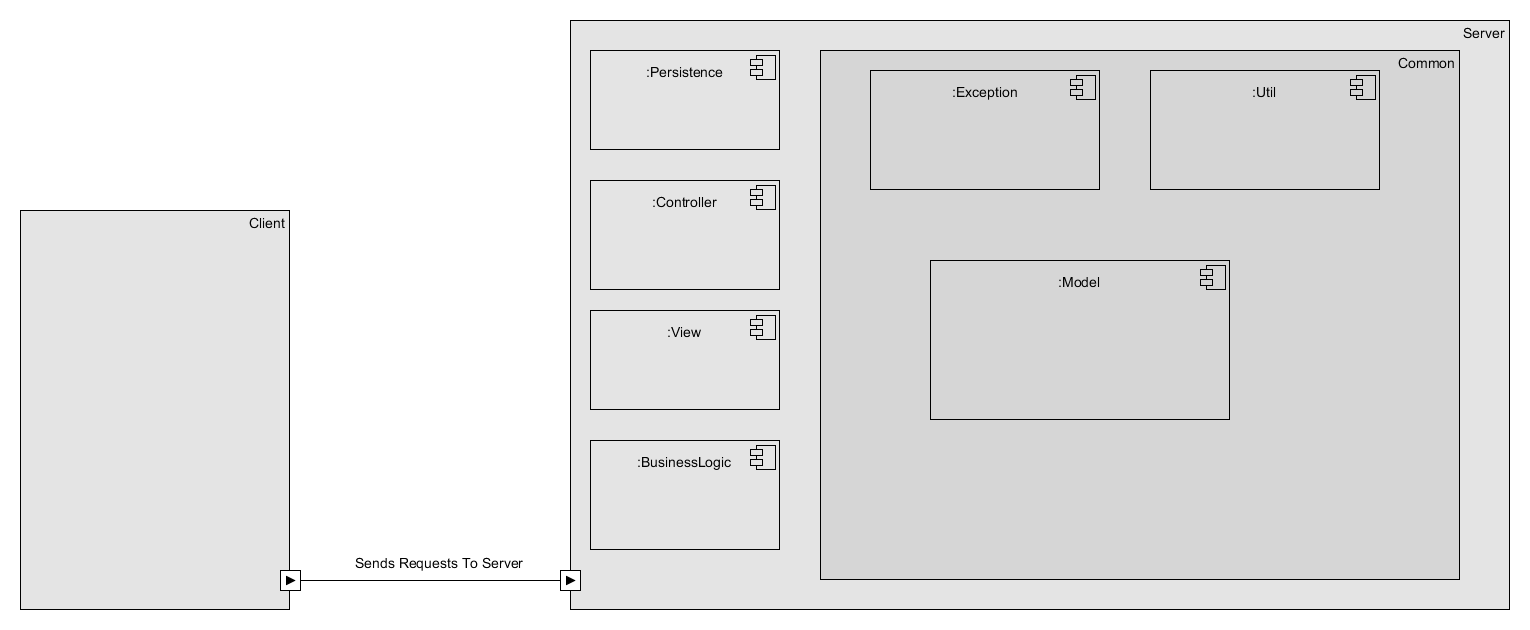
\includegraphics[width=\textwidth,height=15cm,keepaspectratio]{../UMLDiagramme/A-Sicht}
	\caption{Konzeptionelle Sicht - Komponentendiagramm}
	\label{fig15}
\end{figure}
Die Abbildung \ref{fig15} zeigt das Laufzeitverhalten des Systems.\\
Die Interaktion mit dem Softwaresystem erfolgt über eine klassische Client-Server-Struktur.  Es gibt einen Server und beliebig viele Clients, die mit dem Server interagieren. Der Server beinhaltet alle Komponenten des Softwaresystems und der Server verarbeitet die Requests der Clients.   \\
Der Benutzer greift über seinen Browser (Client) auf die Website zu. Die angesteuerte Website ist die index.xhtml. Dabei erhält der Nutzer eine eigene Session. Auf der index.xhtml kann sich der Nutzer einloggen und weitere Teile des Softwaresystems erreichen.
Die Ausführungssicht beinhaltet alle in den vorherigen Sichten getroffenen Entscheidungen. Daher gibt es die aufgeführten Pakete in der Abbildung \ref{fig15} (Common, Persistence, View, Controller). Dadurch das es keine seperate App für mobile Geräte gibt, ist das Ausführungsverhalten auf allen Geräten gleich. Durch die in der Modulsicht getroffene Entscheidung Daten-Backups anzulegen, werden auf dem Server Backup-Dateien abgelegt. Die Datenbank für das Softwaresystem ist ebenfalls auf dem Server. 

%%%%%%%%%%%%%%%%%%%%%%%%%%%%%%%%%%%%%%%%%%%%%%%%%%%%%%%%%%%%%%%%%%%%%%
\section{Zusammenhänge zwischen Anwendungsfällen und Architektur} \label{sec:zusammenhang}
\sectionmark{Zusammenhänge AF u. Architektur}
\label{sec:anwendungsfaelle}

\textbf{Autor: Torben, Arbnor} 

In diesem Abschnitt behandeln wir unsere zuvor erstellten Anwendungsfälle, indem wir die dazugehörigen Sequenzdiagramme erstellen und diese beschreiben. Dabei wird aufgezeigt, wie der Nachrichtenverkehr zwischen allen im Anwendungsfall beteiligten Modulen abläuft.

Bei der Erstellung der folgenden Sequenzdiagramme haben wir die Software Quick Sequence Diagramm Editor verwendet. Wir haben uns für die Notation an die im Rahmen der Softwareprojekt 1-Vorlesung und Tutorium vorgestellten Notation gehalten und können in den Vorlesungsfolien von Prof.Dr.Rainer Koschke zu Softwareprojekt 1 im Sommersemester 2017 eingesehen werden.

\subsection{Anwendungsfall D1: Login als Prüfling}
Der Prüfling ruft die Webseite auf, die per Default unsere  \texttt {Index.html} ist, auf den der Benutzer seinen Usernamen und das Passwort setzten kann. Zunächst wird über index.xhtml über getLanguage() die Sprache geholt. Danach wird zunächst ein neues  \texttt {LoginBean} instanziiert, mit der davor instanziierten  \texttt {Session} und der dazugehörigen  \texttt {UserDAO}. Für den Loginwerden die Methoden setUsername() und setPassword() aus der  \texttt {LoginBean} Klasse aufgerufen. Per Klick auf den Button "Einloggen", wird in der  \texttt {LoginBean} die Methode login aufgerufen, die zunächst abgfragt, ob der Benutzer überhaupt schon eingeloggt ist. Da der Benutzer noch nicht eingeloggt ist, wird False zurückgegeben. In der Annahme, dass der Benutzer nicht null ist, wird letztendlich der String  \texttt {dashboard.xhtml}zurückgegeben, das dazu führt, dass der  \texttt {User} sich nach erfolgreichem Login direkt auf seinem Dashboard befindet.

\begin{figure}[H]
	\centering
	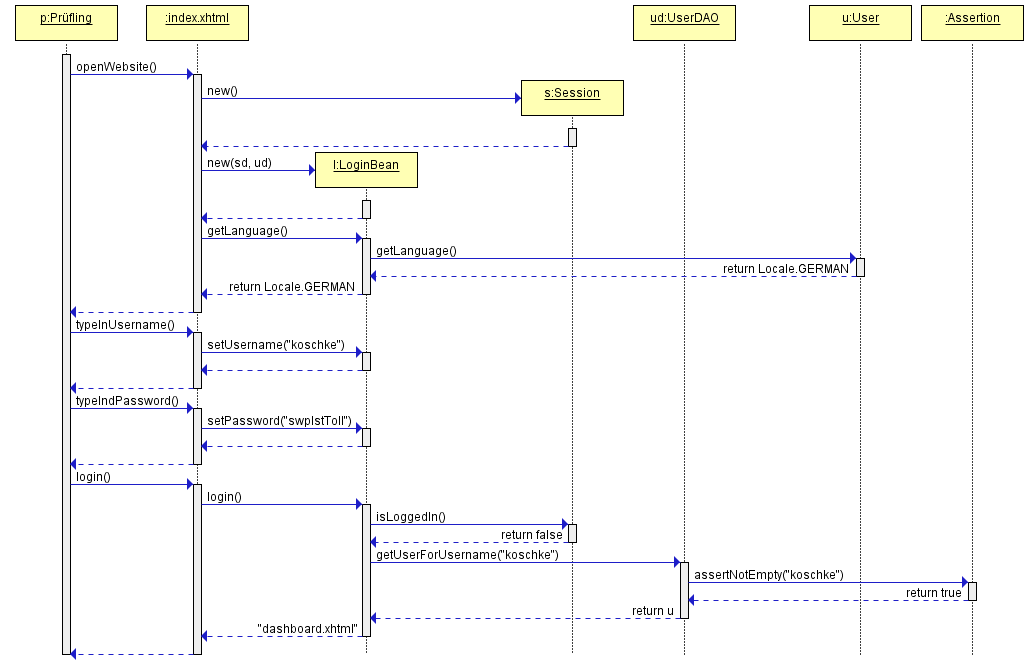
\includegraphics[width=\textwidth,height=15cm,keepaspectratio]{../UMLDiagramme/d1_login}
	\caption{Anwendungsfall D1 : Login als Prüfling}
	\label{fig1}
\end{figure}



\subsection{Anwendungsfall D55: Passwort-Vergessen-Funktion}
Bis zu dem Punkt das eine neue \texttt {LoginBean} instanziiert wird, läuft dieser Sequenzdiagramm gleich, wie das zuvor vorgestellte Diagramm, ab.
Über die  forgotPassword() wird aus der index.html eine neue \texttt {ForgotPasswordBean} instanziiert mit der Session und der MessageDao als Parameter. Dafür wird zunächst die zum Passwort zugehörige Email vom Benutzer in der GUI eingetippt. Mittels setEmail aus \texttt {ForgotPasswordBean}, die aus der \texttt {index.html}  aufgerufen wird, wird die Email gesetzt.
Außerdem wird über die GUI die Martikelnummer vom Benutzer eingetippt und mittels setMatrNr() über \texttt {ForgotPasswordBean} gesetzt.

Sobald die erforderlichen Daten eingetippt und gesetzt sind, kann über den sendPassword-Button in der GUI, welcher sendPassword aus \texttt {ForgotPasswordBean} aufruft, geklickt werden. Dabei verhält sich sendPassword folgendermaßen.
Aus der \texttt {UserDAO} wird mit der übergebenen Email der User aus der Datenbank geladen, und zwar mittels Methodenaufruf getUserForEmail(). Danach wird für den geladenen User mittels getPassword() das Passwort geladen. Damit haben wir alle benötigten Informationen, die wir dem User als Nachricht zusenden können.

Also wird eine neue Nachricht instanziiert, wobei der Empfänger, der Inhalt und der Betreff  durch die \texttt {ForgotPasswordBean} im \texttt {Message}-Objekt gesetzt werden.
Schließlich wird die Nachricht  mittels send() versendet, und mittels save() gespeichert. Schlussendlich wird ein String zurückgegeben, dass die Nachricht versendet wurde. In unserem Fall lautet die Nachricht "Passwort wurde versendet".

\begin{figure}[H]
	\centering
	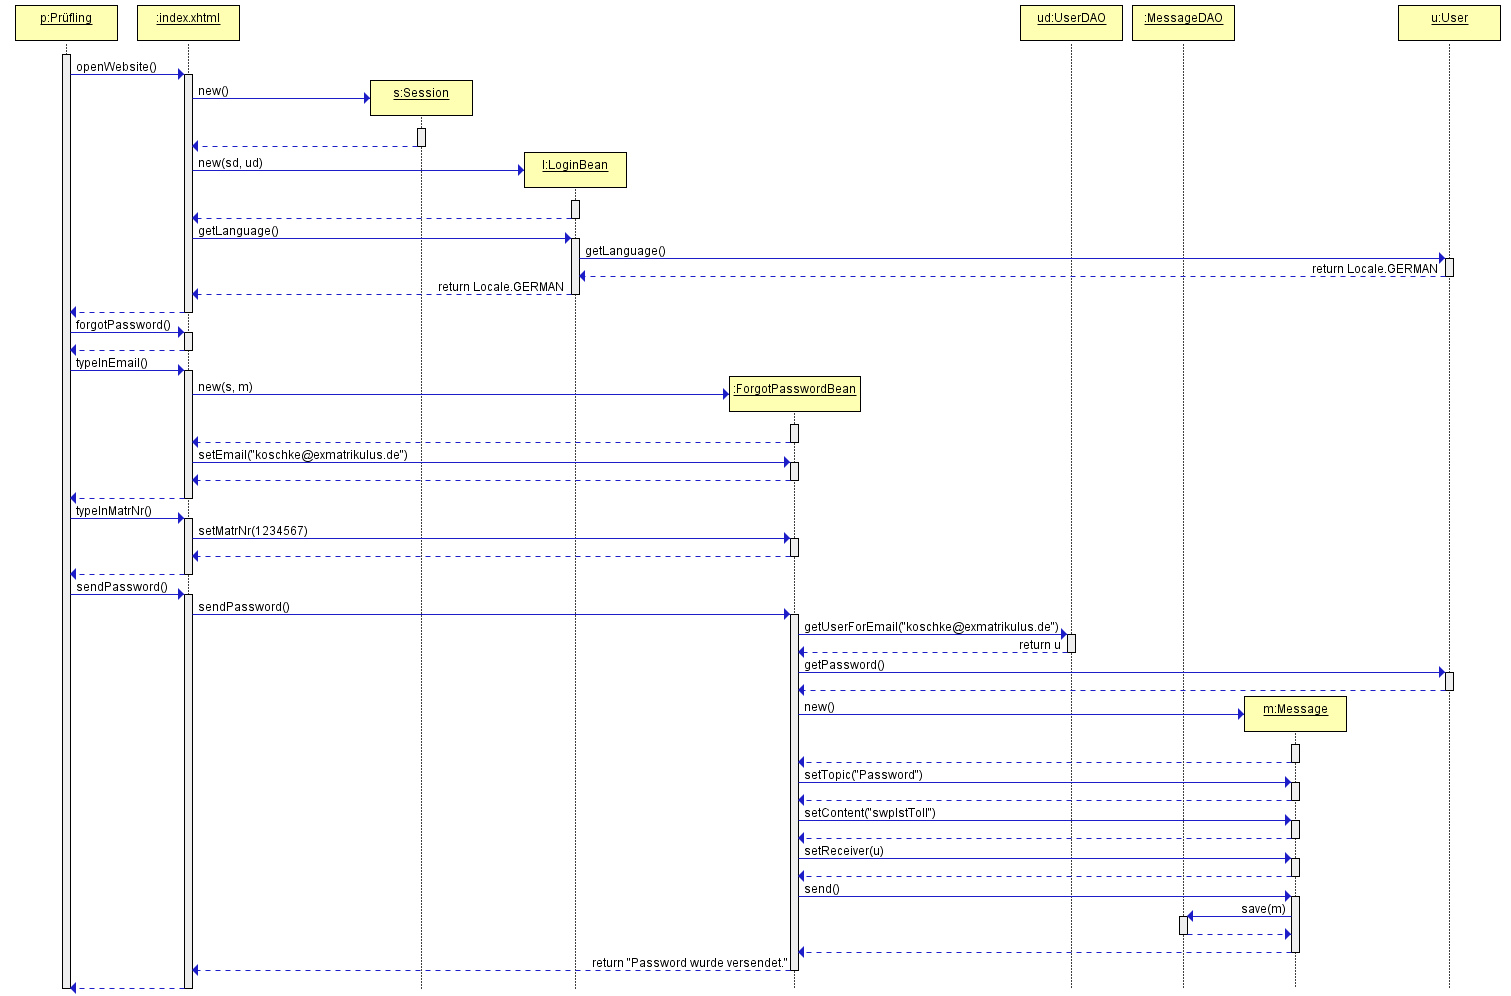
\includegraphics[width=\textwidth,height=15cm,keepaspectratio]{../UMLDiagramme/d55_forgotPassword.png}
	\caption{Anwendungsfall D55 : Passwort-Vergessen-Funktion}
	\label{fig1}
\end{figure}


\subsection{Anwendungsfall D24: Prüfungstermin festlegen}

Über die GUI wird eine neue Prüfung für die Lehrveranstaltung erstellt, die über die Bean \texttt {LectureInstanceExamBean} gesteuert wird. Bei der Erstellung einer neuen Prüfung wird ein neues Objekt vom Typ \texttt {Exam} erstellt, dabei werden alle benötigten Attribute gesetzt, wie dem Datum, der Länge, den Prüfer usw.
Am Ende wird das neue Objekt (die Prüfung) in der DAO über save abgespeichert und die ILV wird geupdated. 


\begin{figure}[H]
	\centering
	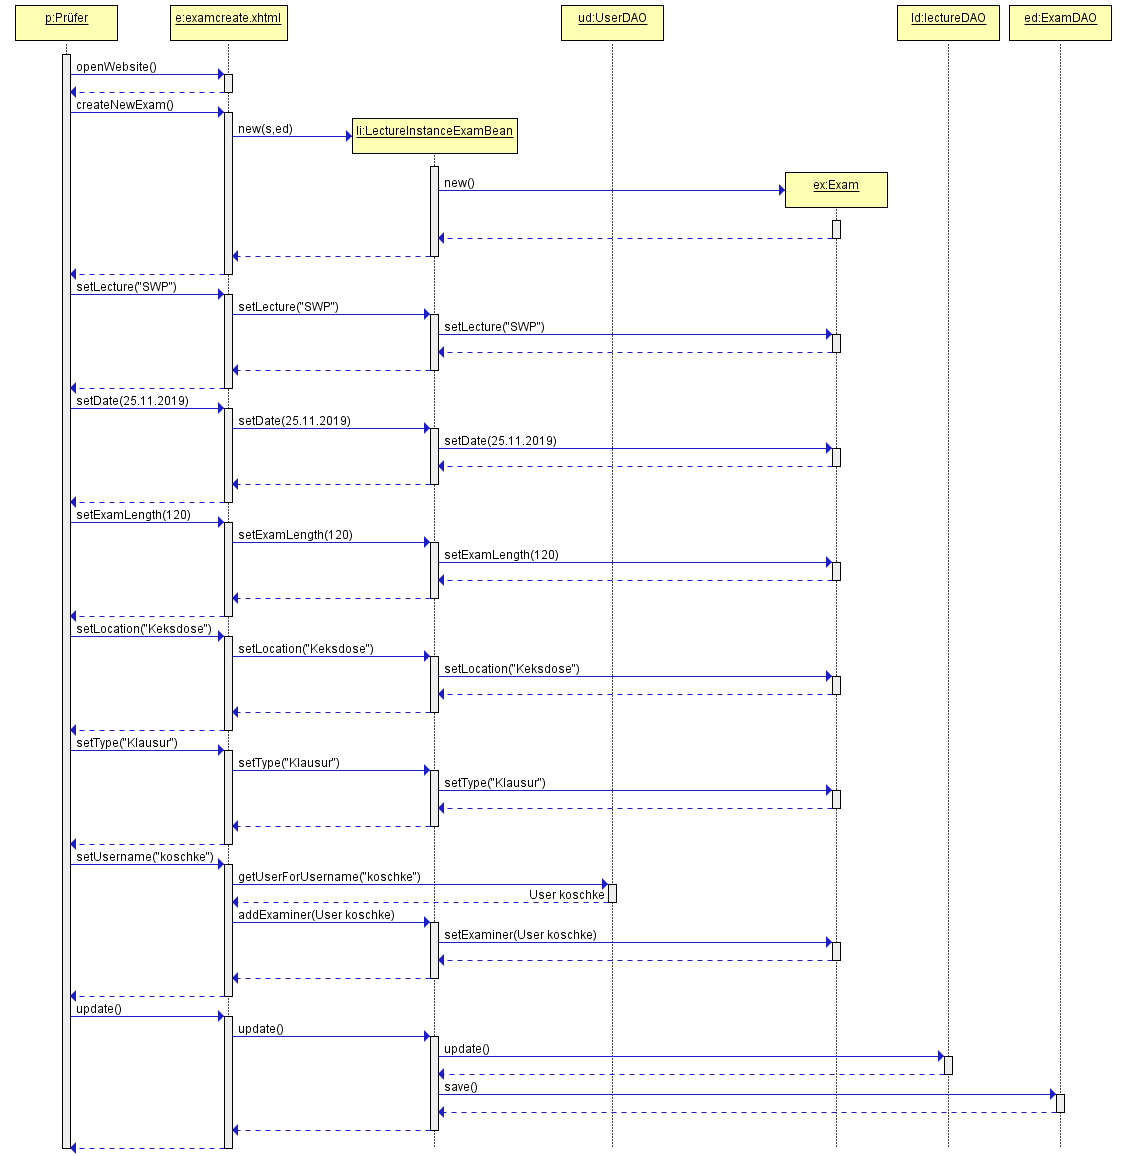
\includegraphics[width=\textwidth,height=15cm,keepaspectratio]{../UMLDiagramme/d24_pruefungstermineFestlegen.png}
	\caption{Anwendungsfall D24 : Prüfungstermin festlegen}
	\label{fig1}
\end{figure}








%%%%%%%%%%%%%%%%%%%%%%%%%%%%%%%%%%%%%%%%%%%%%%%%%%%%%%%%%%%%%%%%%%%%%%
\section{Evolution} \label{sec:evolution}
\textbf{Autor: Anil}\\
Im Folgenden werden mögliche Weiterentwicklungen des Softwaresystems \glqq{}Grade+\grqq{} erläutert und die spezifischen Stellen in der Software genannt, die im Falle von geänderten Anforderungen oder Rahmenbedingungen, geändert werden müssten.\\

\subsection{HTTPS}
Momentan wird  \glqq{}Grade+\grqq{} ohne Hypertext Transfer Protocol Secure (HTTPS) betrieben. 
Jedoch wird für den Betrieb des Systems der Umstieg auf HTTPS  dringend empfohlen. Datensicherheit spielt für den Kunden und die Öffentlichkeit eine wichtige Rolle und HTTPS unterstüzt diesen Wunsch durch besser geschützte Datenübertragungen. Es wurde  bisher nicht implementiert, da aktuell nur lokale Server benutzt wurden. 

\subsection{Andere Datenbank anbinden}
Falls die Datenbank des Softwaresystems nachträglich geändert werden soll, müsste man nur die Komponente Persistence anpassen.
Dort müssten die Methodenzugriffe auf die neue Datenbank angepasst werden. Es sind nur wenige Änderungen erforderlich, da die Komponente als Interface zur Datenbankbank entworfen wurde mithilfe von JPA.

\subsection{Andere Kalender anbinden}
Für das Anbinden von weiteren Kalendern müsste man die Klasse CalendarBean (siehe Abbildung \ref{cal}) anpassen. Dort wird aktuell nur die Implementierung für den Google Kalendar erfolgen. Für weitere  Kalender sollte am besten ein Interface erstellt werden, welche für jeden Kalendar implementiert wird. Die Userprofile müssen angepasst werden, um die Zugangsdaten für weitere Kalendar hinterlegen zu können. Die View müsste um weitere Icons ergänzt werden, damit die anderen Kalendar ausgewählt werden können.

\subsection{Rolle des Sekretärs einbauen}
Die Rolle des Sekretärs wurde bisher nicht eingebaut. Der Sekretär soll den Prüfer unterstützen, wobe er nicht die selben Befugnisse wie ein Prüfer hat.
Es müsste die Rolle des Sektretärs in der Datenbank hinzugefügt werden. Die Zugriffsrechte müssten für jede View  und Bean angepasst werden. Die genauen Zugriffe und und verfügbaren Methoden müsssten für den Sekretär konfiguriert werden. Der Sekretär ist Teil des Chinese Menu.

\subsection{Mobiler Client}
Aus der Problemkarte und unser dazu gehörigen ausgewählten Strategie S10 (Siehe Kapitel \ref{K5} Problemkarte K3) haben wir zunächst auf einen zusätzlichen mobilen Client verzichtet und haben uns für das responsive-Design entschieden.  Die Weiterentwicklung dieser Software, würde für uns bedeuten, dass man eine zusätzliche App für die mobilen Geräte entwickeln könnte. Der mobile Client würde auf die index.xhtml verweisen. In der bestehenden Software müsste man keine Änderungen vornehmen. Alle Seiten der View würden sich aufgrund des responsiven Designs nahtlos in die App integrieren lassen.






\end{document}

%%% Local Variables: 
%%% mode: latex
%%% mode: reftex
%%% mode: flyspell
%%% ispell-local-dictionary: "de_DE"
%%% TeX-master: t
%%% End: 
